%%%--------------------------------%%%
%%% Domain
%%%--------------------------------%%%

\section{User Feedback}
\label{sec:DomainA}
To validate the conclusions we drew from literature research we also gathered potential user feedback to guide our development efforts. First we conducted a short survey to figure out which phases of the risk management process and which platforms we should pay special attention to. We then developed an interactive mock-up to illustrate the core functionality of our application and did some user interviews based on that. We used the feedback to determine the focus areas and features of the application.
\subsection{Survey}
\label{sec:DomainAa}
The survey was conducted among project managers in two big German IT companies. The first sample was collected in December 2019 and amounted to ten answers. The second sample was gathered in January 2020 and contains of 18 project managers. Due to the small sample size our results are not generalizable. To draw any scientific conclusion the findings would have to be verified with a larger sample. However the results are still useful for guiding our development efforts.

We asked the PMs about their previous project experiences in terms of risk managment practice and risks encountered. We also included questions about the importance of different risk managment phases and the usefullness of tool support for them. Finally we gathered information about the platforms they used and on which they would want a risk managment tool. The full questionnaire can be found in the appendix.

The majority of the PMs we surveyed did undertake risk managment efforts for their projects which they oversaw during the last year. Those who did not mostly cited project size as their reason, however some said they usually didn't do it and two even thought it not useful at all as can be seen in FIG.\ref{fig:label20} and FIG.\ref{fig:label21}. We take from that the PMs are generally aware and do undertake risk management efforts given sufficent project volume.

\begin{figure}[H]
	\centering
	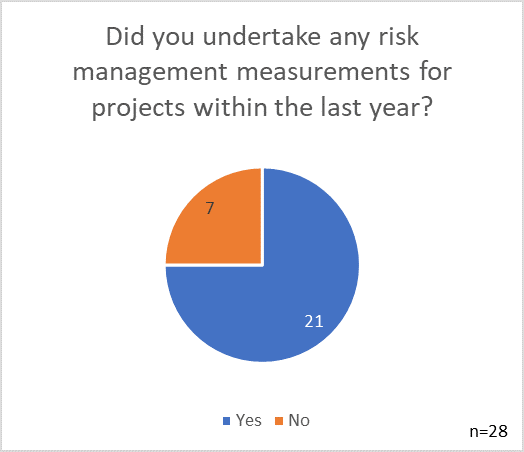
\includegraphics[width=0.6\textwidth]{Assets/survey_results/Q1.png}
	\caption{Engagement in risk management}
	\label{fig:label20}
\end{figure}
\begin{figure}[H]
	\centering
	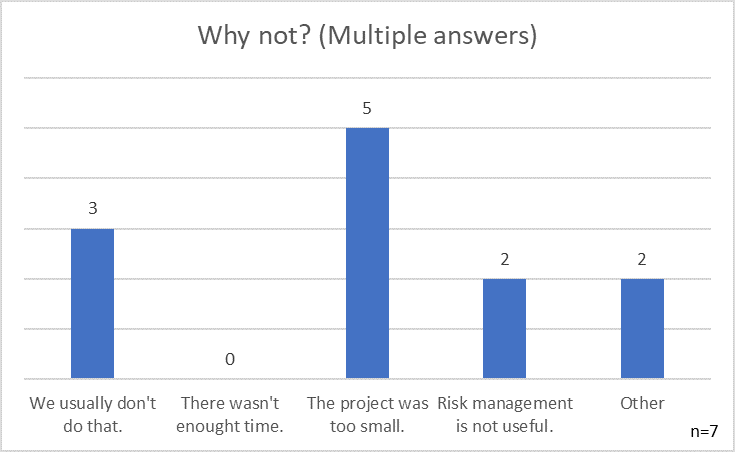
\includegraphics[width=0.6\textwidth]{Assets/survey_results/Q2.png}
	\caption{Reasons for no engagement}
	\label{fig:label21}
\end{figure}

In accordance with the literature all participants who did undertake risk management made an initial commtiment to risk analysis but fewer reported to have to have engange in long term activities for risk monitoring and controlling as depicted in FIG.\ref{fig:label22}. Also when asked about the importance of the different phases the PMs placed a stronger emphasis on the initial phases. Knowing and understanding the risks seem to appear slightly more important than actually dealing with it over the course of the project (see FIG.\ref{fig:label23}).  We therefore believe it is necessary to re-engage the project members throughout the project lifetime so that the less practiced phases of risk management are not overlooked. As argued in the beginning all stages are relevant and should be supported by the software.
 
\begin{figure}[H]
	\centering
	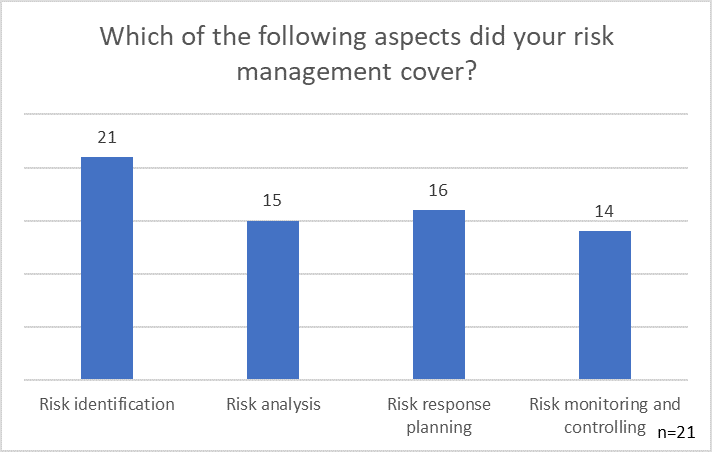
\includegraphics[width=0.6\textwidth]{Assets/survey_results/Q3.png}
	\caption{Engagement across process stages}
	\label{fig:label22}
\end{figure}
\begin{figure}[H]
	\centering
	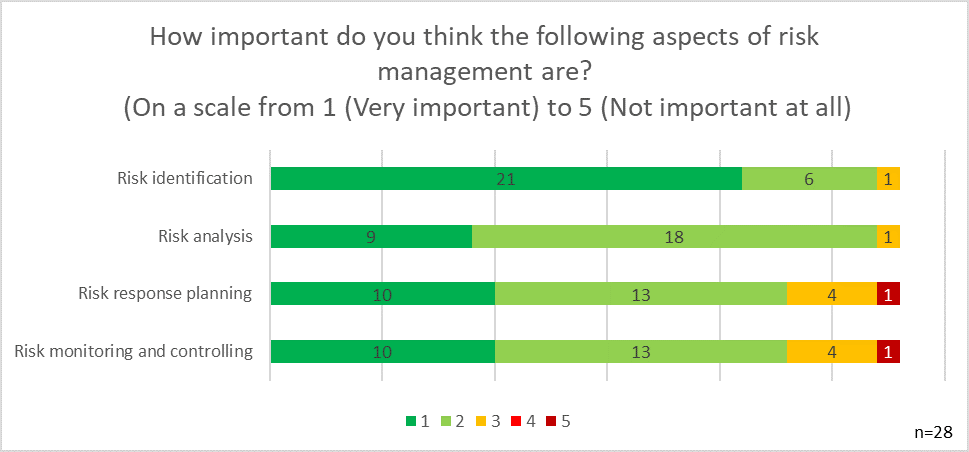
\includegraphics[width=0.6\textwidth]{Assets/survey_results/Q4.png}
	\caption{Importance of process stages}
	\label{fig:label23}
\end{figure}

We also found that the project managers in general were open towards software support for risk management. Many had already used a tool for their efforts and those who didn't were mostly open to the idea (see FIG.\ref{fig:label24}). Some used specific risk management softwares whereas others had customized excel sheets. We thus assume that our chances to gain acceptance for our software are high as long as we provide a good user experience because the PMS are in general open to software support.

\begin{figure}[H]
	\centering
	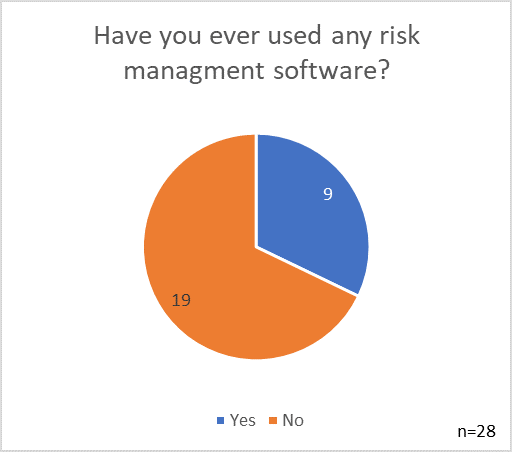
\includegraphics[width=.45\textwidth]{Assets/survey_results/Q5.png}
	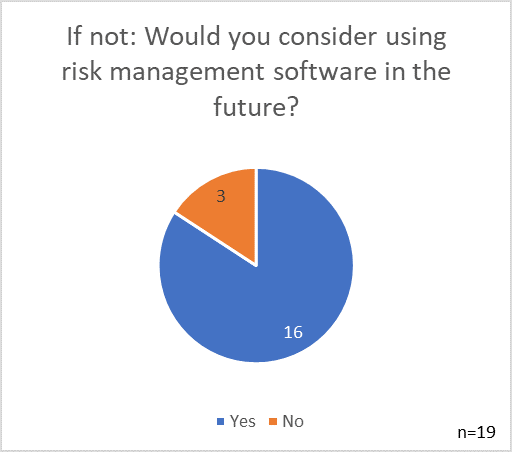
\includegraphics[width=.45\textwidth]{Assets/survey_results/Q6.png}
	\caption{Willingness to use software for risk management efforts}
	\label{fig:label24}
\end{figure}

We again find our conclusion supported that risk managment software can be especially useful for keeping efforts alive long-term with the next survey question. We specifically asked the PMS who were open for tool support which phase of the process would in their eyes benefit most from tool support\footnote{Unfortunately filtering issues occured at the second company for the last questions which is why not all participants who should have received the question can be reported.}. Monitoring and controlling is the most frequently picked option as FIG.\ref{fig:label25} shows. 

\begin{figure}[H]
	\centering
	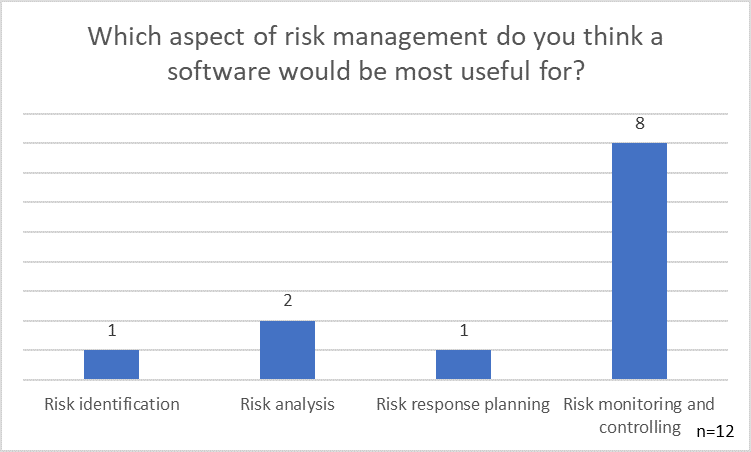
\includegraphics[width=0.6\textwidth]{Assets/survey_results/Q8.png}
	\caption{Tool usefulness across process stages}
	\label{fig:label25}
\end{figure}

Finally we asked the PMs on which platforms they would want to use a risk management tool on (see FIG.\ref{fig:label26}). Mainly they preferred desktop computers with different operating systems (MacOS, Windows and Linux were all mentioned). Roughly a third would also like to have a mobile solution, however. It is noteworth that all who picked mobile also chose desktop aswell. From this question we derive that our PWA approach is a good way to cover all usage preferences.

\begin{figure}[H]
	\centering
	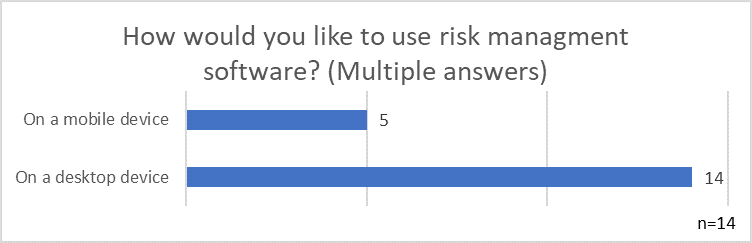
\includegraphics[width=0.6\textwidth]{Assets/survey_results/Q7.png}
	\caption{Grouped answers: Platform preference for tool usage}
	\label{fig:label26}
\end{figure}

From these results we developed a basic clickable prototype of the software which can be found at: \underline{\href{https://norisknofun.invisionapp.com/prototype/NoRiskNoFunPreview-ck5aubx9g002w6o01rhyo61z3/play/40faaf12}{No Risk No Fun - Interactive Prototype}}. It is an initial sketch of how we intended to realize the above described conclusions in our software. We used the prototype to gain further feedback for refining our designs. This feedback can be found in the following section, the refined software specifications are described in \ref{sec:domainB}.

\subsection{Interviews}
\label{sec:DomainAb}
For the interviews we managed to secure further support from the company surveyed in December. Three project managers agreed to test our mock-up prototype and give us feedback. Two of the PMs were male, one was female. All three were provided with a convertible device and requested to explore the prototype while thinking out loud. We asked them to speak out whatever came to their minds while using the mock-ups and to pose any questions that came up. Afterwards we asked them for their overall assessment of the tool, which parts of it they deemed useful and where it was lacking.

All project managers rated the tool as useful for risk management efforts though for different reasons. Two of them said it was helpful in focusing their activities. One said that usually risk management was more of a minor activity that happened on the side. The other described the initally discussed pattern of risk management happening at the beginning of the project and then being neglected, forgotton or tedious to come back to. He expected that activity tracking and easy notification of team members via delibarte push notifications could actually turn risk managment into a process instead of a one-time activity. This supports our focus on motivation and long term commitment.

The third PM was more skeptical of these kinds of features. He said that with some or perhaps more considerable effort he could build such a process into his task managing tool and thus preferred not having to manage two tools. However, he saw much use in the risk pool feature which collects and persists the experience of many projects and thus would provide valuable guidance. The risk pool was also deemed useful by the other two PMs. We thus conclude that the risk pool is pracitcable way to adress the need of documentation and knowledge persistance identified in \ref{sec:theoryAd}.

All PMs also appreciated that risk evaluation was a group task and not determined by individual opinions. The fact that adjustment and re-opening of risk evaluation was possible after the inital risk assessment.

All three PMS requested more visual reporting aid to gain a clearer view of project health status. We take from it, that the activity graph does not sufficently cover the need for visualization and that further reporting graphics should be devised.

Furthermore some functionalities or positioning was not understood, which we will work on improving in the actual application. Also many small additional features were suggested which are listed in the appedix for future expansion.
